%!TEX root = Slic3r-Manual.tex

\subsection{\texttt{Extrusion Width}} % (fold)
\label{sec:extrusion_width}
\index{extrusion width}

\begin{figure}[H]
\centering
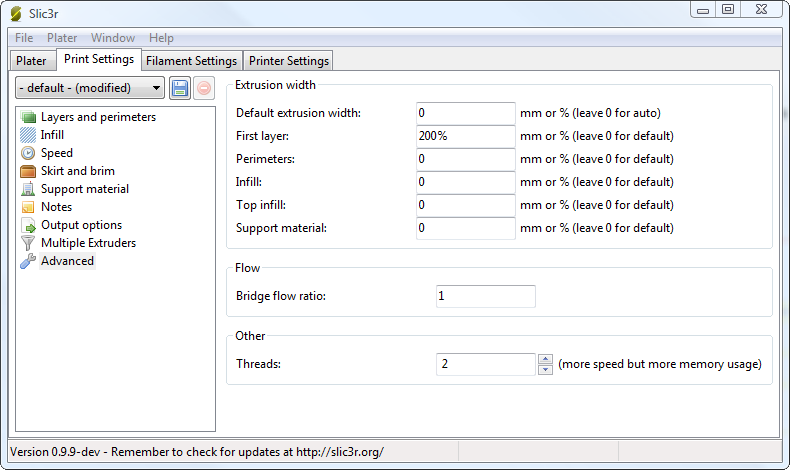
\includegraphics[keepaspectratio=true,width=1\textwidth]{expertmode/advanced_extrusion_widths_options.png}
\caption{Extrusion widths options.}
\label{fig:advanced_extrusion_widths_options}
\end{figure}

One reason for modifying the extrusion width has already been discussed: increasing first layer extrusion width in order to improve bed adhesion (see p.\pageref{par:wider_extrusion_width}).  There are some further cases where it may be beneficial to modify extrusion widths.
\begin{itemize}
    \item \texttt{Perimeter} - A lower value will produce thinner extrusions which in turn will produce more accurate surfaces.
    \item \texttt{Infill} and \texttt{Solid Infill} - A thicker extrusion for infill will produce faster prints and stronger parts.
    \item \texttt{Top infill} - A thinner extrusion will improve surface finish and ensure corners are tightly filled.
    \item \texttt{Support material} - As with the infill options, a thicker extrusion will speed up print time.
\end{itemize}

It is important to remember that if the extrusion width is expressed as a percentage then this is computed from the \texttt{Layer height} property, and not the \texttt{Default extrusion width} setting.

% subsection extrusion_width (end)
